\section[Lokalisierung (Niklas Schäfer)]{Lokalisierung\begin{tiny} (Niklas Schäfer)\end{tiny}}
\subsection{Einleitung}
Essentiell für die Auswertung eines Erdbebens mit Smartphones ist die Lokalisierung. Empfängt der Server Alarme von Smartphones, ist es notwendig, dass er unter anderem auch die Standortdaten von der App geliefert bekommt. Zum einen benötigt man eine Lokalisierung um feststellen zu können wo sich das Beben befindet und zum Anderen muss der Server anhand der Standorte der empfangenen Alarme auswerten können, ob es sich um einen korrekten Alarm oder einen Fehlalarm handelt.
Zum Beispiel ist es möglich, dass das Fahren in einem Bus den Beschleunigungssensor Bewegungen wahrnehmen lässt, die einem Erdbeben ähnlich sind, sodass die App von einem Erdbeben ausgehen muss und einen Alarm an den Server sendet. Da der Server bei Alarmen immer durch Mehrheitsentscheidung urteilt, könnte es passieren, dass er auf ein Erdbeben schließt, wenn mehrere Personen in einem Bus fahren. Daher muss gewährleistet werden, dass es mindestens einen Alarm gibt, der einen bestimmten Mindestabstand zu den betreffenden anderen Alarmen hat.

\subsection{Location Provider des Android-Systems}\label{subsec:locProvider}
Im Android System gibt es drei unterschiedliche Location Provider (Verfahren und Sensoren die einen Standort bestimmen können), die Positionsdaten eines Android Smartphones liefern können:

\begin{itemize}
     \item PASSIVE
     \item NETWORK
     \item GPS
\end{itemize}

\subsubsection{PASSIVE}
Der Location Provider PASSIVE initialisiert keinen Zugriff auf einen der vorhandenen Sensoren des Smartphones. Er nutzt lediglich den zuletzt abgerufenen Standort, der sich noch im Speicher des Android Systems befindet. Das heisst, dass er nur den Standort liefert, der von irgendeiner anderen App oder dem Android System selbst zu irgendeinem Zeitpunkt über die Location Provider NETWORK oder GPS abgerufen worden ist. Der Vorteil des PASSIVE Providers liegt darin, dass er keinen Sensor abfragen muss, sondern lediglich den Speicher ausliest und daher sehr stromsparend fungiert. Für die Quakedetec App ist er allerdings nicht sinnvoll verwendbar, da man keinen ausreichend aktuellen Standort erhält. Es ist beispielsweise möglich, dass die letzte Sensorabfrage schon sehr lange zurück liegt und der Standort veraltet ist.
Somit wäre eine Erdbebenlokalisierung fehlerhaft.

\subsubsection{NETWORK}
Der Location Provider NETWORK findet Positionsdaten mit Hilfe von WLan-Netzwerken und der Mobilfunkzelle (\shorthandoff{"}"Mobilfunkmast"\shorthandon{"}). 
Um über WLan-Netzwerke Geräte lokalisieren zu können, pflegt Google eine Datenbank, die WLan-Netzwerke mit Standortdaten verknüpft.
Anfangs geschah dies mit Hilfe des Google Fahrzeugs, welches hauptsächlich zur Datenerfassung für Google StreetView in vielen Städten unterwegs war. Hierbei erfasste dieses Fahrzeug auch WLan-Netze und verknüpfte deren MAC-Adresse mit den GPS Daten des Fahrzeugs.
Natürlich sind solche Daten schnell veraltet, weshalb Google weitherin Android Smartphones nutzt um die Daten aktuell zu halten und neue WLan-Netze in die Datenbank aufzunehmen.
Android Smartphones übermitteln dabei ihren GPS Standort zusammen mit den MAC Ids der sichtbaren WLan Netzwerke in ihrer Umgebung an Google. Dabei wird auch die Signalstärke der WLan-Netzwerke berücksichtigt um den Standort des WLan-Netzwerks noch genauer ermitteln zu können.
Um einen Standort über den NETWORK Provider abzurufen, sendet das Smartphone einen \textit{Request} an Google. In diesem \textit{Request} sind die MAC Ids  und Signalstärken der WLan-Netze enthalten, die gerade für das Smartphone sichtbar sind. Es werden alle WLan Netze und deren Signalstärken von Google benötigt um einen noch genaueren Standort bestimmen zu können. Würde man nur das verbundene WLan übermitteln, könnte man nur den Standort des einzelnen WLan Netzes zur Ermittlung des Standorts des Gerätes verwenden. Hat dieses WLan Netz eine hohe Signalstärke, sodass es in einem Radius von mehreren hundert Metern empfangbar ist, wäre der Standort auch nur auf mehrere hundert Meter genau. Bezieht man aber mehrere WLan Netzwerke mit ein, kann man durch die Überschneidungen der Netze den Standort wesentlich genauer bestimmen. 

\begin{figure}[H]
	\centering
	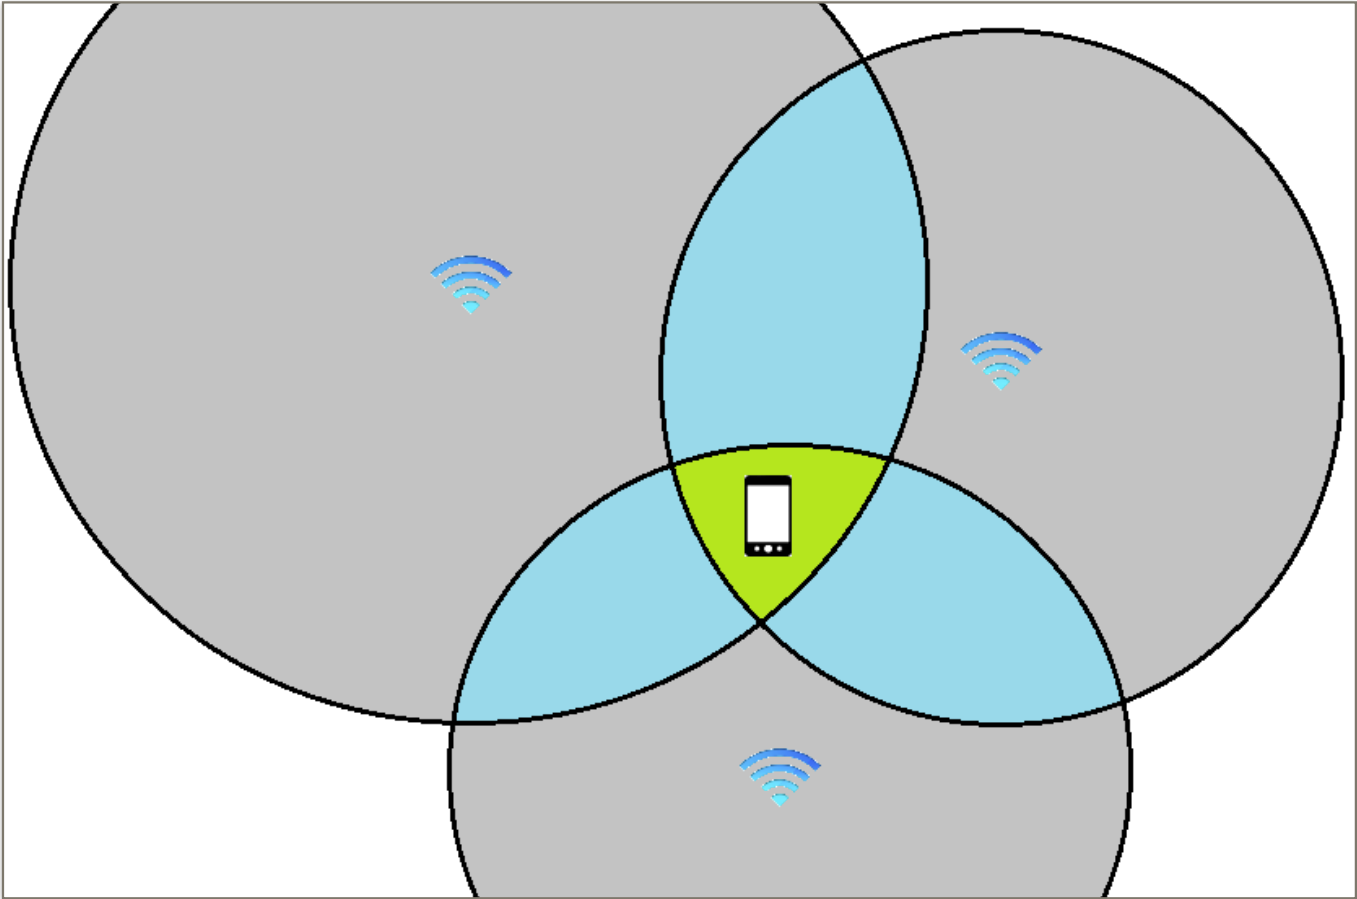
\includegraphics[width=130mm]{/network_provider.png}
	\caption[Lokalisierung: Lokalisierung mit NETWORK Provider]{Lokalisierung mit NETWORK Provider}
	\label{fig:networkProviderfunc}
\end{figure}

In Abbildung \ref{fig:networkProviderfunc} ist die Funktionsweise dieser Lokalisierungstechnik skizzenhaft dargestellt. Ist am Standort allerdings nur ein WLan Netzwerk sichtbar, bezieht Google zum Teil die Signalstärke mit ein, wodurch auch in diesem Fall die Genauigkeit noch ein wenig verbessert wird.
Wurde der Request vom Smartphone an den Google Server übergeben, werden anhand der gesendeten MAC IDs die verfügbaren Standorte der umgebenen WLan Netze aus der Google Datenbank entnommen. Daraufhin wird ein Standort mit der beschriebenen Funktionsweise ermittelt (Überschneidungen) und an das Smartphone zurückgesendet. Die Antwort vom Google Server beinhaltet den Längen- und Breitengrad und die Genauigkeit des gelieferten Standorts. 
Die Genauigkeit dieses Verfahrens liegt erfahrungsgemäß zwischen 15-100m.

\begin{figure}[H]
\centering
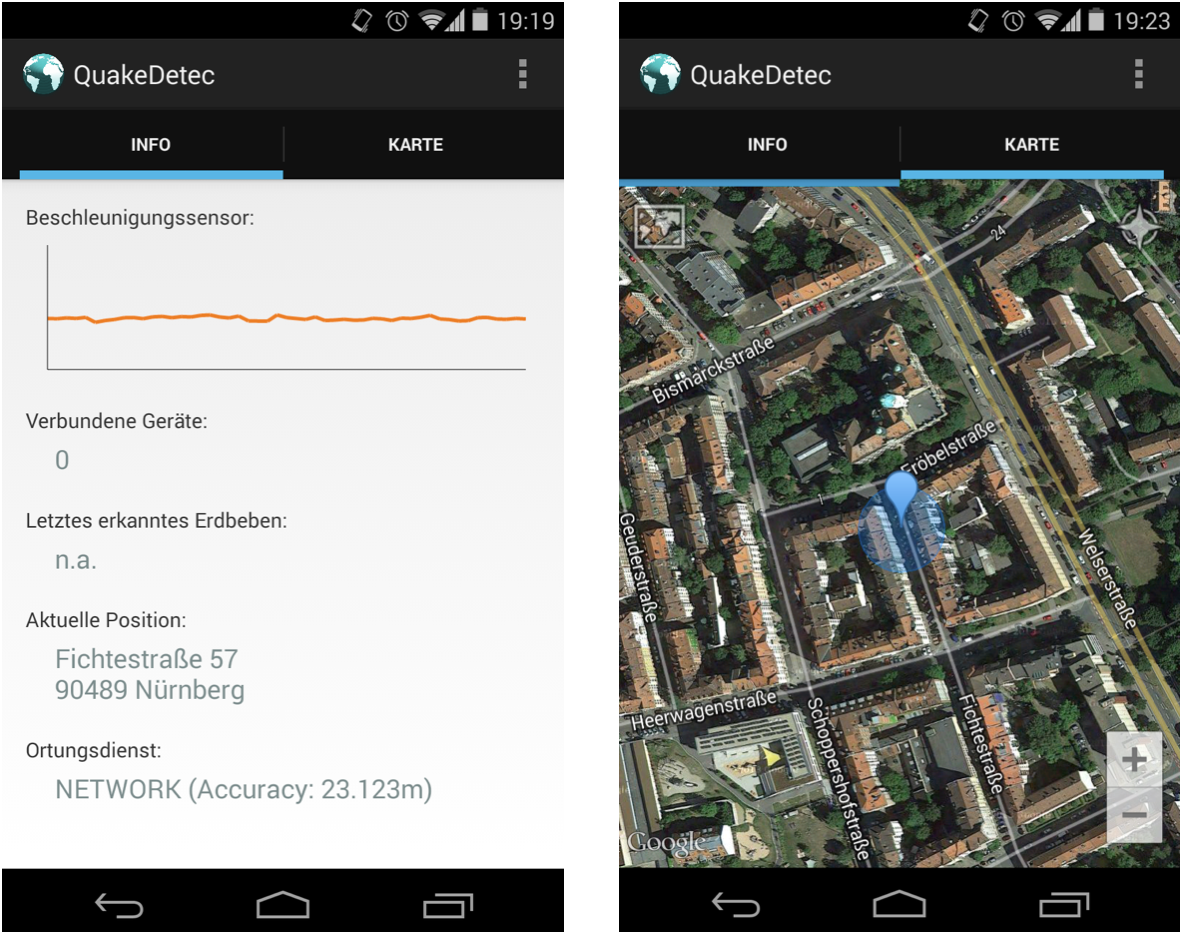
\includegraphics[width=\textwidth]{/network_provider_gui.png}
\caption[Lokalisierung: User Interface bei Nutzung des NETWORK Providers]{User Interface bei Nutzung des NETWORK Providers}
\label{fig:networkProviderGui}
\end{figure}

Sollten keine WLan-Netzwerke verfügbar oder das WLan des Smartphones deaktiviert sein, nutzt der NETWORK Provider die Mobilfunkzellen zur Ortsbestimmung. Dies funktioniert im Grunde nach dem selben Prinzip wie die Lokalisierung über WLan-Netze, allerdings werden hierbei keine Überschneidungen mehrerer Mobilfunkzellen berücksichtig. Dazu müsste man das sogenannte Timing-Advance Verfahren verwenden. Bei diesem Verfahren wird der Standort ermittelt indem Signallaufzeiten zum verbundenen Mobilfunkmast gemessen werden. Berechnet man nur die Signallaufzeit zu einem Mast, kann man nur bestimmen auf welchem Radius sich das Gerät befindet. Um den Standort mit Hilfe von Signallaufzeiten genauer zu bestimmen, ist es notwendig die Signallaufzeit zu einem weiteren Mobilfunkmast zu messen.

\begin{figure}[H]
\centering
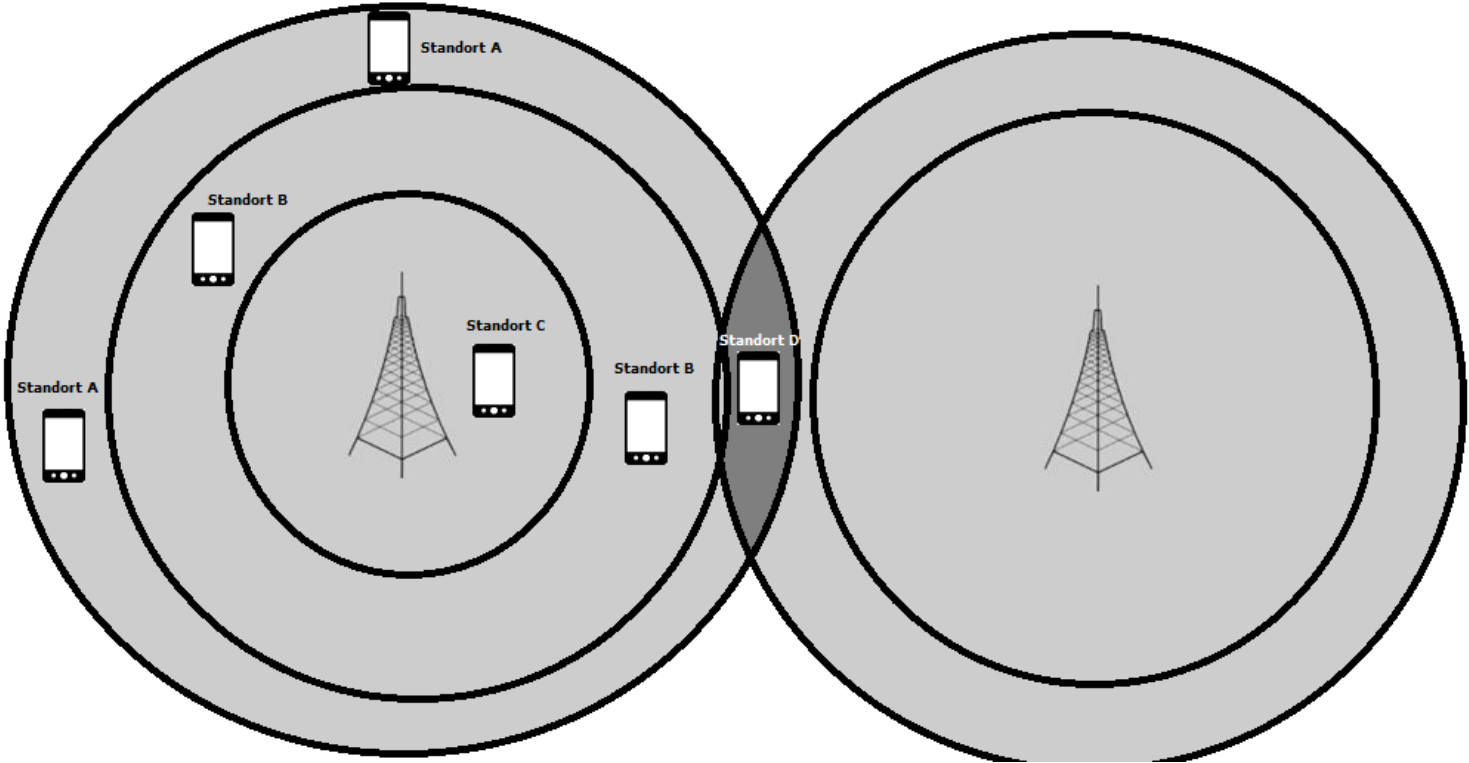
\includegraphics[width=\textwidth]{/network_provider_timing_advance.png}
\caption[Lokalisierung: Timing-Advance Verfahren]{Timing-Advance Verfahren}
\label{fig:networkProviderTimingAdvance}
\end{figure}

Damit hat man zwei Radien, die sich schneiden und man kann relativ genau den Standort ermitteln. 

\begin{wrapfigure}{r}{43mm}
\centering
   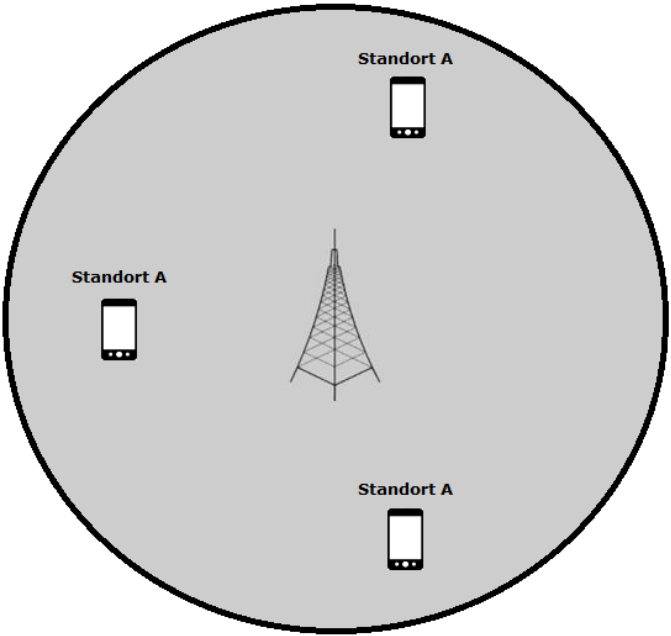
\includegraphics[width=43mm]{/network_provider_praxis.png} 
   \caption[Lokalisierung: NETWORK Provider in der Praxis]{Praxis}
\end{wrapfigure}

Dieses Verfahren findet allerdings kaum Verwendung, da man das Gerät dazu zwingen muss die Verbindung zwischen  mehreren Mobilfunkzellen zu wechseln um in jeder Zelle die Signallaufzeit zu messen. Dieser Vorgang führt schnell zu einem hohen Energieverbrauch.
Somit wird in der Praxis eine Lokalisierung nur mit Hilfe einer einzigen Mobilfunkzelle durchgeführt. 

Eine Mobilfunkzelle hat eine vielfach höhere Signalreichweite als ein WLan-Netzwerk. In Städten liegt man hier zwar nur bei wenigen hundert Metern, auf dem Land hingegen bei mehreren Kilometern. Somit erhält man in der Stadt meist noch Standortdaten, die auf wenige hundert Meter genau sind, auf dem Land liegt man allerdings meist bei 2 bis 4 Kilometer.

\subsubsection{Global Positioning System}
Mittlerweile besitzt fast jedes aktuelle Android Smartphone einen GPS-Empfänger. 
Das Global Positioning System wurde vom amerikanischen Verteigungsministerium entwickelt. Es besteht aus 30 Satelliten, welche die Erde umkreisen und Nachrichten aussenden, die zur Positionsbestimmung eines Empfängers dienen. Das Global Positioning System ist vom Prinzip her der Positionsbestimmung über Mobilfunkzellen im Timing-Advance Modus ähnlich. 
Ein Satellit sendet eine Nachricht mit seiner Position und zu welchem Zeitpunkt die Nachricht versendet wurde kontinuierlich aus.
Ein GPS-Empfänger kann aus der Versandzeit einer Nachricht die Signallaufzeit bestimmen (aktuelle Zeit - Versandzeit = Signallaufzeit). Aufgrund der Signallaufzeit kann somit bestimmt werden, auf welchem Radius sich der Empfänger vom Satelliten befindet. 
\begin{wrapfigure}{r}{55mm}
\centering
   \begin{center}
   	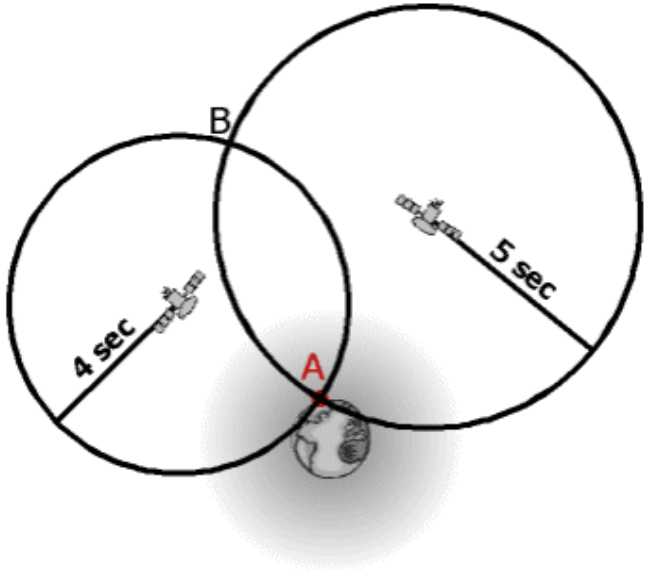
\includegraphics[width=55mm]{/gps_two_satellites.png} 
   \end{center}
   \caption[Lokalisierung: GPS 2 Satelliten]{GPS 2 Satelliten}
   \label{fig:gpsTwoSatellites}
\end{wrapfigure}
Ein einziger Satellit würde zu einer genauen Positionsbestimmung nicht ausreichen, da man im Grunde nur die Entfernung zu diesem einen Satelliten bestimmen kann. Nutzt man aber mehrere Satelliten, kann man die Überschneidungen der Radien nutzen, um die Position sehr genau zu bestimmen. Mit zwei Satelliten kann man theoretisch in einer zwei-dimensionalen Welt schon eine Position bestimmen. In Abbildung \ref{fig:gpsTwoSatellites} ist ein Beispiel mit zwei Satelliten zu sehen. Hat man zwei Satelliten und somit zwei Radien, schneiden sich diese zwei Radien in zwei Punkten. Da aber einer dieser Punkte weit im Weltall liegt, kann man schnell darauf schließen, dass nur der andere Relevant und somit der eigene Standort ist. In einer zwei-dimensionalen Ebene braucht man in der Realität allerdings noch einen dritten Satelliten um das sogenannte Uhrenproblem zu lösen. Die Satellitenuhren laufen zwar dank Atomuhren absolut genau und synchron, ein GPS-Empfänger tut dies allerdings nicht. Dadurch würden die Signallaufzeiten bei zwei Satelliten ungenau berechnet werden. 

Zieht man einen dritten Satelliten heran, kann man dieses Problem lösen. 
\begin{wrapfigure}{l}{48mm}
	\centering
	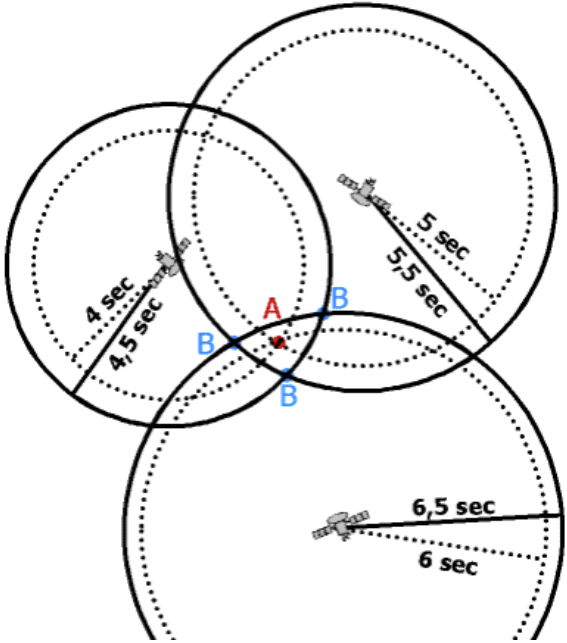
\includegraphics[width=48mm]{/gps_three_satellites.png}
	\caption[Lokalisierung: GPS 3 Satelliten]{GPS 3 Satellites}
	\label{fig:gpsThreeSatellites}
\end{wrapfigure}
Abbildung \ref{fig:gpsThreeSatellites} verdeutlicht die Funktionsweise. Unter der Annahme, dass die Empfängeruhr 0,5s vorgeht, bekommt man Radien die aufgrund der falsch laufenden Empfängeruhr größer ausfallen (durchgezogene Linien/Kreise). In der Realität sind diese aber kleiner (gepunktete Linien/Kreise). Bei zwei Radien hätte man immer noch zwei Schnittpunkte der Radien, die dann allerdings eine falsche Position angeben würden. Zieht man allerdings einen dritten Satelliten zur Bestimmung heran, hat man bei einer falschen Berechnung aufgrund des Uhrenproblems keinen Schnittpunkt aller drei Radien. In diesem Fall verändert der GPS-Empfänger seine Uhrzeit so lange, bis sich alle drei Radien in einem Punkt schneiden. Somit wird die Uhrzeit des GPS-Empfängers mit der Uhrzeit der Satelliten synchronisiert. Der Schnittpunkt aller drei Radien ist dann die exakte Position.
Zur Realisierung dieses Systems und zur genauen Bestimmung der Position in der Realität, also in einer drei-Dimensionalen Welt, wird noch ein vierter Satellit verwendet. Dies ist notwendig, da in der hier beschriebenen Funktionsweise von einem zwei-dimensionalen Modell ausgegangen wird. Man kann mit diesem Modell zwar auch die Position in der Realität bestimmen, allerdings geht man dabei davon aus, dass sich die zu bestimmende Position auf Meereshöhe befindet. Somit wäre eine Positionsbestimmung falsch, sobald sich der Empfänger über dem Meerespiegel befindet.
Bei der drei-dimensionalen Positionsbestimmung wird dieses Problem mit einem vierten Satelliten gelöst. Mit diesem ist es auch möglich die Höhe des Empfängers zu bestimmen. Allerdings soll hier nicht weiter darauf eingangen werden. Dazu der Verweis auf andere Informationsquellen.

\subsection{Positionsbestimmung in Android}\label{subsec:posInAndroid}

Wie schon in Kapitel~\ref{subsec:locProvider} beschrieben, bietet das Android System drei Möglichkeiten um den Standort zu bestimmen. Um unter Android diese Möglichkeiten zu nutzen, bietet die Android API die drei Locationprovider PASSIVE, NETWORK und GPS.
Um einer App den Zugriff auf diese Provider zu gewähren, muss der Zugriff erstmal vom Nutzer erfragt und gewährt werden. Um diese Berechtigung vor der Installation beim Nutzer einzuholen, muss man folgende Codezeile im Android-Manifest hinzufügen:

\begin{lstlisting}[caption={App Permissions},label=lst:locationPermission]
<manifest ... >
    <uses-permission android:name="android.permission.ACCESS_FINE_LOCATION" />
    ...
</manifest>
\end{lstlisting}

Möchte ein Nutzer die App nun installieren, wird er zuerst gefragt, ob er der App den Zugriff auf die Standortdaten seines Geräts gewähren möchte. Es ist zwingend erfordlich, dass die Abfrage akzeptiert wird, ansonsten wird die App nicht installiert.

\begin{figure}[H]
	\centering
	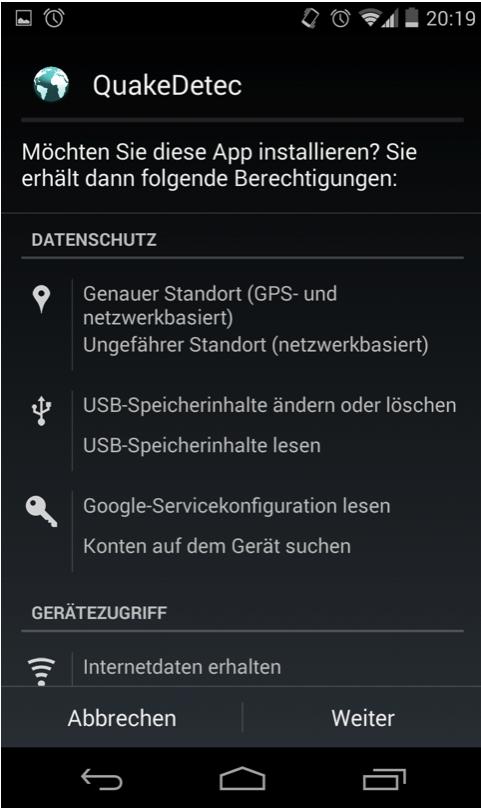
\includegraphics[width=40mm]{/app_permissions.png}
	\caption[Lokalisierung: App Permissions]{App Permissions}
	\label{fig:appPermissions}
\end{figure}

Um in der App auf die Location Provider zugreifen zu können, benötigt man eine Instanz des Android \textit{LocationManagers}. Mit diesem ist es möglich auf die Location Services zuzugreifen und eine Standortbestimmung auszulösen.

Eine Instanz des LocationManagers erlangt man durch folgende Codezeile:

\begin{lstlisting}[caption={LocationManager Instanz},label=lst:locationManagerInstance, basicstyle=\footnotesize]
// Acquire a reference to the system Location Manager
LocationManager locationManager = (LocationManager) this.getSystemService(Context.LOCATION_SERVICE);
\end{lstlisting}

Außerdem sind LocationListener notwendig, welche beschreiben, wie auf bestimmte Ereignisse der Location Services reagiert werden soll.

Es gibt vier Ereignisse auf die reagiert werden kann:
\begin{itemize}
     \item Neuer Standort
     \item Provider aktiviert
     \item Provider deaktiviert
     \item Status der Provider hat sich geändert
\end{itemize}
Die entsprechenden Methoden des Listeners sind:
\begin{itemize}
     \item \textit{onLocationChanged(Location location)}
     \item \textit{onProviderEnabled(String provider)}
     \item \textit{onProviderDisabled(String provider)}
     \item \textit{onStatusChanged(String provider, int status, Bundle extras)}
\end{itemize}
Hat beispielsweise ein Sensor einen neuen Standort registriert, wird die \textit{onLocationChanged} Methode aufgerufen, der ein Location Objekt übergeben wird. In diesem Objekt ist der Längen- und Breitengrad, die Genauigkeit des Standortes in Metern und der Location Provider, der den Standort ermittelte, enthalten. 
\\
Wird ein Location Provider (z.B. GPS) im System deaktiviert, wird die \textit{onProviderDisabled} (bzw. wenn aktiviert \textit{onProviderEnabled}) Methode mit dem Providernamen als Parameter aufgerufen und man kann dementsprechend in der App darauf reagieren. 

\newpage
Das vierte Ereignis auf das reagiert werden kann, ist eine Statusänderung eines Location Providers. Wenn ein Provider aus irgendeinem Grund nicht verfügbar war und wieder verfügbar wird, wird \textit{onStatusChanged} aufgerufen.

\begin{lstlisting}[caption={LocationListener},label=lst:locationListener]
// Define a listener that responds to location updates
LocationListener locationListener = new LocationListener() {
    public void onLocationChanged(Location location) {
      // Called when a new location is found by the network location provider.
      makeUseOfNewLocation(location);
    }
    public void onStatusChanged(String provider, int status, Bundle extras) {}
    public void onProviderEnabled(String provider) {}
    public void onProviderDisabled(String provider) {}
  };
\end{lstlisting}

Um Standortdaten abzufragen, gibt es zwei Möglichkeiten. 
Eine ist kontinuierlich auf Standortänderungen zu reagieren. Das heißt, dass Standortänderungen zu jedem Zeitpunkt wahrgenommen werden.

\begin{lstlisting}[caption={requestLocationUpdates},label=lst:requestLocationUpdates, basicstyle=\small]
locationManager.requestLocationUpdates(LocationManager.NETWORK_PROVIDER, time, distance, locationListener);
\end{lstlisting}

Dieser Methode wird unter anderem der \textit{Location Provider} und der entsprechende \textit{LocationListener} übergeben. Ein weiterer Parameter steht für die Zeit, die vergangen sein muss, bis wieder ein neuer Standort zurückgegeben wird. Gibt man zum Beispiel 10 Minuten an, wird für 10 Minuten kein neuer Standort zurückgegeben. 
Der letzte verbleibende Parameter steht für die Distanz, die überbrückt worden sein muss, bis ein neuer Standort zurückgegeben wird. Setzt man diesen Parameter zum Beispiel auf 100m, wird ein neu erkannter Standort nur zurückgegeben, wenn sich dieser mindestens 100m vom alten Standort entfernt befindet. 
\\
\\
Eine andere Möglichkeit einen Standort zu ermitteln ist ein ein einmaliger Abruf des aktuellen Standorts.
\begin{lstlisting}[caption={requestSingleUpdate},label=lst:requestSingleUpdate, basicstyle=\small]
locationManager.requestSingleUpdate(LocationManager.NETWORK_PROVIDER, locationListener, looper);
\end{lstlisting}


Dieser Methode wird ebenfalls der \textit{LocationListener} und der gewünschte \textit{Location Provider} übergeben. Zusätzlich wird bei dieser Methode noch ein Looper Objekt benötigt. Dieses wird benötigt um Messages in Queues auszuführen. 
Diese Methode aktiviert den gewünschten Location Provider und wartet bis ein Standort von diesem zurückgegeben wurde. Danach wird der Location Provider wieder deaktiviert und es werden keine neuen Standorte mehr ermittelt.

\subsection{Umsetzung der Quakedetec App}
\subsubsection{Erste Umsetzung und Probleme}
Anfangs wurde die App mit der requestLocationUpdates Methode (siehe Kapitel \ref{subsec:posInAndroid}) und dem NETWORK und GPS Provider umgesetzt. Es wurden beide Sensoren kontinuierlich abgefragt und der genauere

\begin{wrapfigure}{r}{50mm}
\centering
   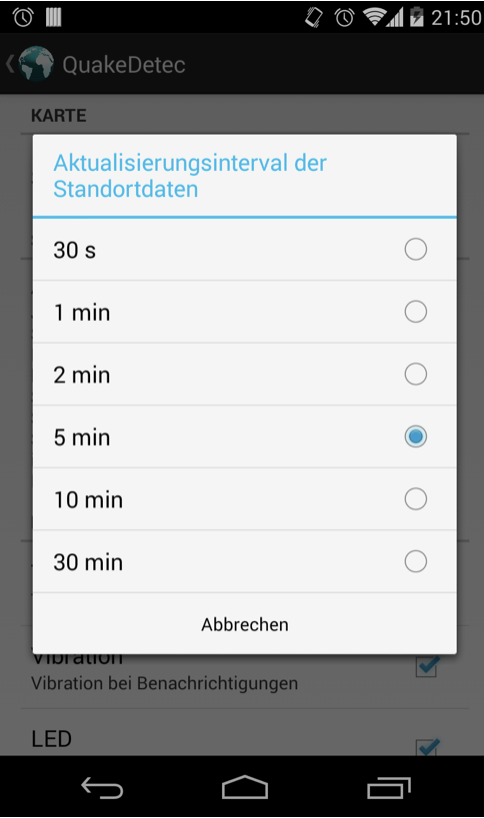
\includegraphics[width=50mm]{/locationupdates_interval_ui.png} 
   \caption[Lokalisierung: Update Interval]{Update Interval}
\end{wrapfigure}

und aktuellere Standort der beiden Location Provider wurde verwendet. Da man im Falle eines Erdbebens den Standort des Geräts benötigt um die Erdbebenposition zu bestimmen, erachteten wir es als sinnvoll, den Standort kontinuierlich zu bestimmen. Diese Möglichkeit bot die requestLocationUpdates Methode. Allerdings fiel schnell auf, dass der Akkuverbrauch mit dieser Lösung sehr hoch und somit inakzeptabel war. Um dieses Problem zu lösen, fügten wir in der App die Einstellung für ein Aktualisierungsinterval hinzu. Über diese Einstellung stellten wir eine Möglichkeit zur Verfügung in der requestLocationUpdates Methode den Parameter für die Zeit zu setzen (in Kapitel \ref{subsec:posInAndroid} beschrieben). Das bot dem Nutzer die Möglichkeit das Zeitinterval zu bestimmen, welches vergangen sein muss bis ein neuer Standort zurückgegeben wird. Zum Zeitpunkt der Implementierung war uns nicht bewusst, dass diese Umsetzung keine Auswirkung auf den hohen Akkuverbrauch haben wird. Denn nicht wie zuerst angenommen, sinkt zwischen dem Intervall der Energieverbrauch der Sensoren, sondern er bleibt identisch, da die Sensoren trotz des Zeitintervals durchgehend aktiv bleiben.
Das heißt, dass der Standort trotz des Intervals durchgehend bestimmt wird, nur dass der Standort ausschließlich nach verstreichen des Intervals zurückgegeben wird.
Als uns dies bewusst wurde, stellten wir die Lokalisierung um auf Singleupdates (\textit{requestSingleUpdate}, siehe Kapitel \ref{subsec:posInAndroid}). Diese Singleupdates wurden mit Hilfe eines Timer Threads, welcher in einem Hintergrundservice läuft, ausgeführt. Nun wurde das Interval dieses Timer Threads über die Einstellung in der App gesetzt. Somit ist dies nun ein reales Interval in dem die Sensoren deaktiviert werden. 
Das brachte zwar eine Verbesserung in der Akkuleistung, aber der Verbrauch war selbst bei einem 10 Minuten Interval noch zu groß. Außerdem war diese Umsetzung nicht vereinbar mit der benötigten Aktualität der Standortdaten. Denn letztendlich kann sich ein Nutzer innerhalb von 10 Minuten schon an einem ganz anderen Standort befinden. Wurde beispielsweise eine Standortaktualisierung 9 Minuten vor einem Erdbebenalarm ausgelöst und der Benutzer war in dieser Zeit in Bewegung, sind die an den Server übermittelten Standortdaten nicht mehr aktuell und können stark von der tatsächlichen Position abweichen. Somit war diese Lösung ebenfalls inaktzeptabel und die Implementierung musste überdacht werden.

\subsubsection{Finale Umsetzung}
Das Problem des hohen Akkuverbrauchs konnte schnell ausfindig gemacht werden. GPS ist zwar mit einer Genauigkeit von drei Metern sehr präzise, aber der GPS Sensor hat einen sehr hohen Akkuverbrauch. Außerdem hat GPS das Problem, dass eine Sichtverbindung zu Satelliten bestehen muss. Somit ist eine Positionsbestimmung innerhalb von Gebäuden mit GPS nicht möglich. Und schließlich werden sich Nutzer überwiegend innerhalb von Gebäuden aufhalten.
Somit entschlossen wir uns, überwiegend auf GPS zu verzichten und primär auf den NETWORK Provider zurückzugreifen. Dieser bietet den Vorteil, dass er sehr stromsparend ist und innerhalb von Gebäuden ebenfalls nutzbar ist. In Städten hat dieser Provider durch die hohe WLan- und Funkzellendichte eine gute Genauigkeit. Bei Tests in Nürnberg lag die Genauigkeit zwischen 20-50m.
\begin{wrapfigure}{r}{60mm}
\centering
   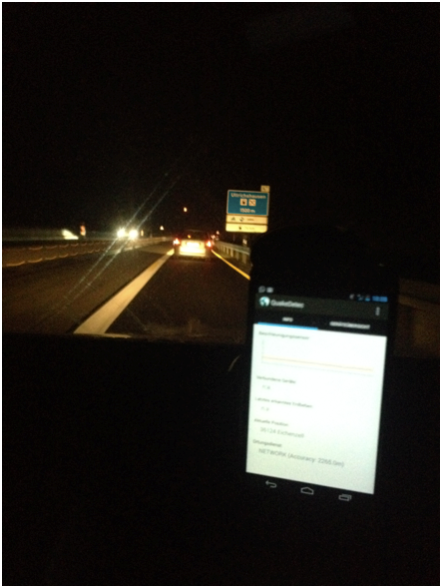
\includegraphics[width=60mm]{/test_autobahn.png} 
   \caption[Lokalisierung: Test auf der Autobahn]{Test auf der Autobahn}
\end{wrapfigure}
Leider hat er den Nachteil, dass er auf dem Land sehr ungenau werden kann, da hier oft keine WLan Netze und nur sehr wenige Funkzellen vorhanden sind. Bei durchgeführten Tests beispielsweise in einem ländlichen Raum in der nähe Bad Hersfelds und auf Autobahnen lagen die schlechtesten Werte bei 3400m. An sich ist dieser Wert kein sehr großes Problem bei der Erdbebenerkennung, allerdings kommt hierbei zum tragen, dass zum Teil mehrere Benutzer in einem Senderadius um einen Funkmast den genau gleichen Standort zugeordnet bekommen können, und zwar den des Funkmasts. Das führt zu der Problematik, dass wir bei einer Erdbebenauswertung (siehe xxx) auf dem Server nicht feststellen können, ob sich die Nutzer genau am selben Standort oder weit voneinander entfernt befinden. Bei der Erdbebenauswertung mit Hilfe einer Mehrheitsentscheidung muss man allerdings ausschließen können, dass sich die Nutzer nicht am gleichen Ort (z.B. in einem Radius von 100m) befinden. Denn sollten z.B. mehrere Nutzer in einem Bus unterwegs sein und aufgrund erdbebenähnlicher Bewegungen des Busses einen Erdbebenalarm an den Server senden, würde bei der Auswertung ein Erdbeben festgestellt werden. Um diesen Fall auszuschließen, wird bei der Erdbebenauswertung immer überprüft, ob mindestens ein Gerät der Alarmauslösenden mindestens 100m von den anderen entfernt ist. Das bedeutet im ländlichen Raum, dass ein Gerät mindestens soweit von den anderen entfernt sein muss, sodass es mit einer anderen Funkzelle verbunden ist. Das heißt bei dem von uns am schlechtest gemessenen Wert von 3400m, dass eines von den alarmauslösenden Geräten mindestens 3401m vom Funkmast entfernt sein muss, damit es einen anderen Standort hat und man sich bei der Auswertung sicher sein kann, dass sich die Geräte nicht am selben Standort befinden. Um zu gewährleisten, dass die Ungenauigkeit nicht zu groß wird, wurde die Lokalisierung so implementiert, dass bei einer Genauigkeit höher als 3500m der GPS Sensor aktiviert wird und über diesen ein genauer Standort abgerufen wird.
Das heißt zusammenfassend, dass die App im worst-case Szenario nur Erdbeben erkennt, die weiter strahlen als 3500m, sodass Geräte in einem Radius, der größer als 3500m ist, das Beben noch wahrnehmen können.
Die Implementierung auf diese Weise stellte den besten Kompromiss zwischen Akkuverbrauch und Genauigkeit dar, da der GPS Sensor somit nur sehr selten verwendet wird.
\par\bigskip
\begin{wrapfigure}{r}{45mm}
	\centering
 	\vspace*{-10mm}
	\label{notification_localizer_app}{
    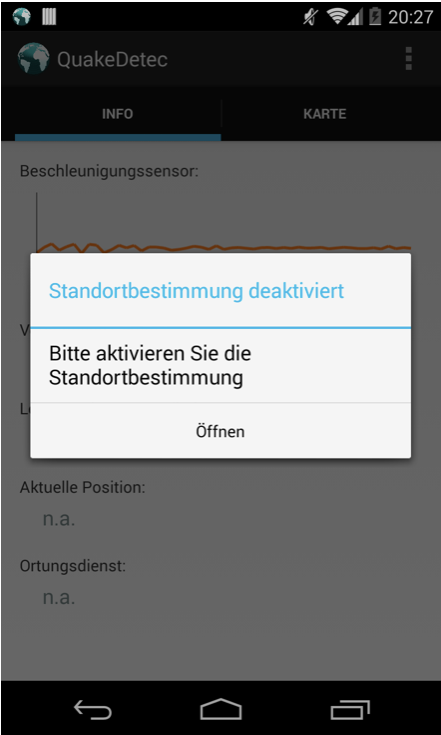
\includegraphics[width=39mm]{/notification_localizer_app.png}}
    \vspace*{-2mm}
    \caption[Lokalisierung: Notification in der App]{Notifications}
	\vspace*{5mm}
	\label{notification_localizer_statusbar}{
    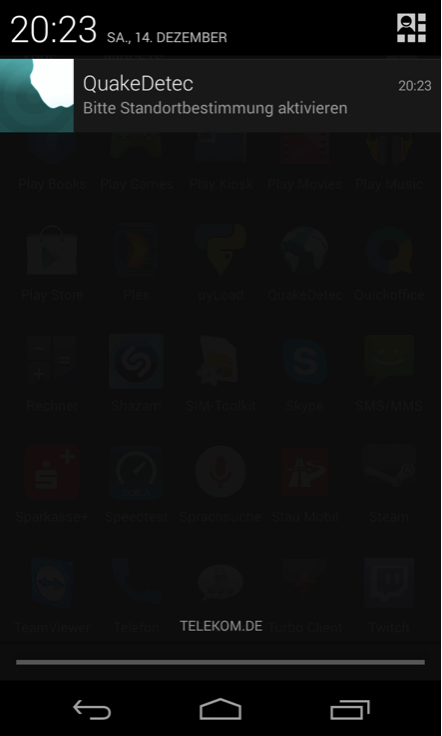
\includegraphics[width=39mm]{/notification_localizer_statusbar.png}}
    \vspace*{-2mm}
    \caption[Lokalisierung: Notification bei geschlossener App]{Notifications}
    \vspace*{-10mm}
\end{wrapfigure}
Da die App abhängig von den Standortdaten ist und ohne Lokalisierung nutzlos ist, prüft die App, ob zumindest eine der beiden Lokalisierungsmethoden (NETWORK oder GPS) im Android System aktiviert ist. Ist dies nicht der Fall, wird bei geöffneter App ein Popup angezeigt, welches den Nutzer auffordert, die  Lokalisierung zu aktivieren. Tippt der Nutzer auf „Öffnen“, werden die Android Systemeinstellungen für die Lokalisierung geöffnet. In der App verschwindet das Popup erst, wenn eine der beiden Lokalisierungsmethoden aktiviert wurde. 
\par\bigskip
Läuft die App im Hintergrund und der Nutzer deaktiviert die Lokalisierung, gibt die App eine Android Notification in der Android Statusbar aus. Diese kann vom Nutzer nicht geschlossen werden und verschwindet ebenfalls erst nach der Aktivierung einer Lokalisierungsmethode.

\par\bigskip
Um das Problem der Aktualität der Daten zu lösen, wurde die Standortabfrage flexibel gestaltet. Ist die App geöffnet und sichtbar, wird die Standortabfrage in einem Intervall von 30s ausgeführt. Das Interval ist bei geöffneter App kurz gewählt, damit gewährleistet wird, dass der Nutzer in der Standortanzeige und der Google Map einen relativ aktuellen Standort angezeigt bekommt. Ist die App nicht sichtbar oder läuft im Hintergrund, wird eine Standortabfrage in einem Interval von 10 Minuten ausgeführt. Diese Abfrage ist notwendig, da die App  alle 10 Minuten einen Heartbeat mit dem Standort an den Server sendet. Außerdem wird ein Standort abgefragt, sobald ein Erdbeben erkannt wurde und wird mit dem Alarm an den Server gesendet. Da ein Alarm in der App zeitkritisch ist und eine Standortabfrage mit Hilfe des GPS Sensors eine längere Zeit beanspruchen kann, wird zusätzlich in einem Interval von fünf Minuten eine Standortabfrage unabhängig vom Heartbeat oder Alarm ausgeführt. Somit kann sichergestellt werden, dass ein Standort der mit einem Alarm gesendet wird, nicht älter als fünf Minuten ist, falls die Standortabfrage unmittelbar vor dem Alarm zuviel Zeit in Anspruch nimmt und nicht auf diese gewartet werden kann.

\subsubsection{Klassendiagramm Localizer}
\begin{figure}[H]
	\centering
	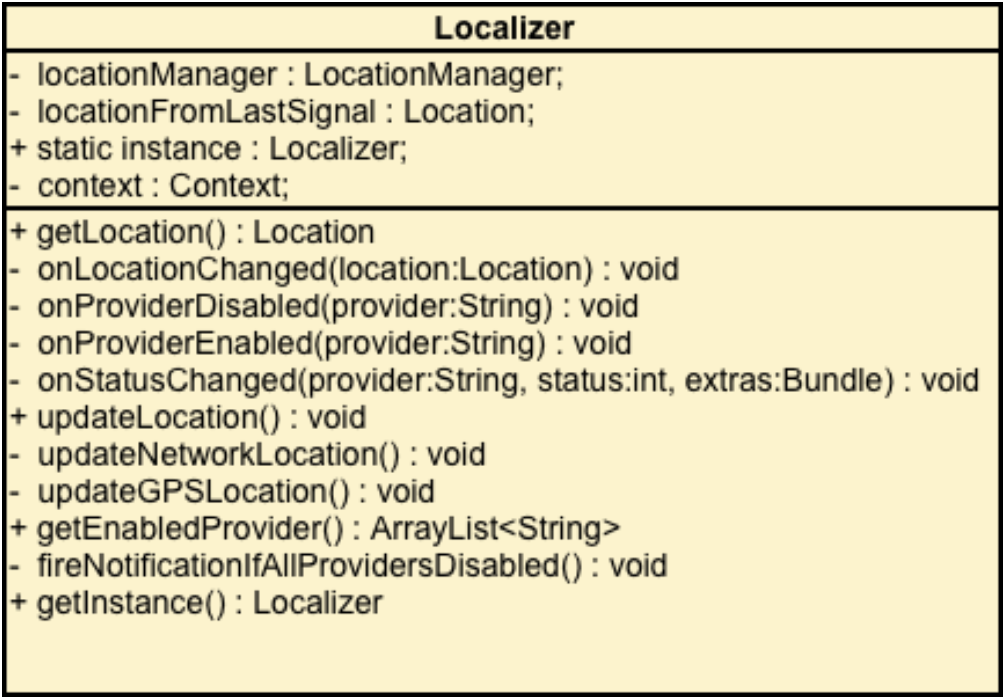
\includegraphics[width=130mm]{/localizer_class.png}
	\caption{Lokalisierung: Localizer}
	\label{fig:localizerClass}
\end{figure}